\documentclass[a4paper,12pt]{article}
\usepackage{graphicx}
\usepackage{hyperref}
\usepackage{geometry}
\usepackage{fancyhdr}
\usepackage{xcolor}
\usepackage{setspace}
\usepackage{enumitem}
\usepackage{titlesec}
\usepackage{helvet} 

\geometry{a4paper, margin=1in}

\definecolor{shakespeareblue}{RGB}{0, 51, 102}
\definecolor{shakespearegreen}{RGB}{44, 117, 52}
\definecolor{shakespeareyellow}{RGB}{255, 204, 0}

\pagestyle{fancy}
\fancyhf{}
\fancyhead[L]{\textbf{\Huge Shakespeare's Cities Visualization}} 
\fancyhead[R]{
\includegraphics[width=2cm]{logo_pant.jpg}}
\fancyfoot[C]{\thepage}

\renewcommand{\rmdefault}{ppl} 
\renewcommand{\sfdefault}{phv} 

\titleformat{\section}[block]{\normalfont\Large\bfseries\color{shakespeareblue}}{\thesection}{1em}{}
\titleformat{\subsection}[runin]{\normalfont\large\bfseries\color{shakespearegreen}}{\thesubsection}{1em}{}
\titleformat{\subsubsection}[runin]{\normalfont\itshape\color{shakespeareyellow}}{\thesubsubsection}{1em}{}

\title{
    \vspace{0cm} 
    \begin{flushleft} 
    \textbf{\huge \sffamily Visualization of Shakespeare's Cities} \\[0.5cm] 
    \end{flushleft}
    \LARGE \textbf{Rrona Abrashi and Qendrese Buza } \\[1cm]
    \textcolor{shakespeareyellow}{\rule{0.8\linewidth}{0.5mm}} \\[1cm]
    \large \textit{January 2025} 
    \vspace{1cm}
}
\author{}
\date{}

\begin{document}

\maketitle

\noindent
\textbf{\huge \color{shakespeareblue} Introduction} \\[0.5cm]
To better understand the geographical range of locations referenced in Shakespeare’s plays, this visualization explores the diverse settings used throughout his works. By using interactive mapping tools, we can chart out the cities and regions that shaped his stories, bringing new insights into his writing and the cultural landscape of the Elizabethan era. The goal is to explore how Shakespeare’s imagination traveled far beyond England to places like Italy, Denmark, and Greece, influencing some of his most iconic plays. This project uses modern tools such as \textbf{RStudio} and the \texttt{leaflet} package to bridge the past and present, offering a visual experience of Shakespeare’s global worldview.

\vspace{1cm}

\begin{center}
    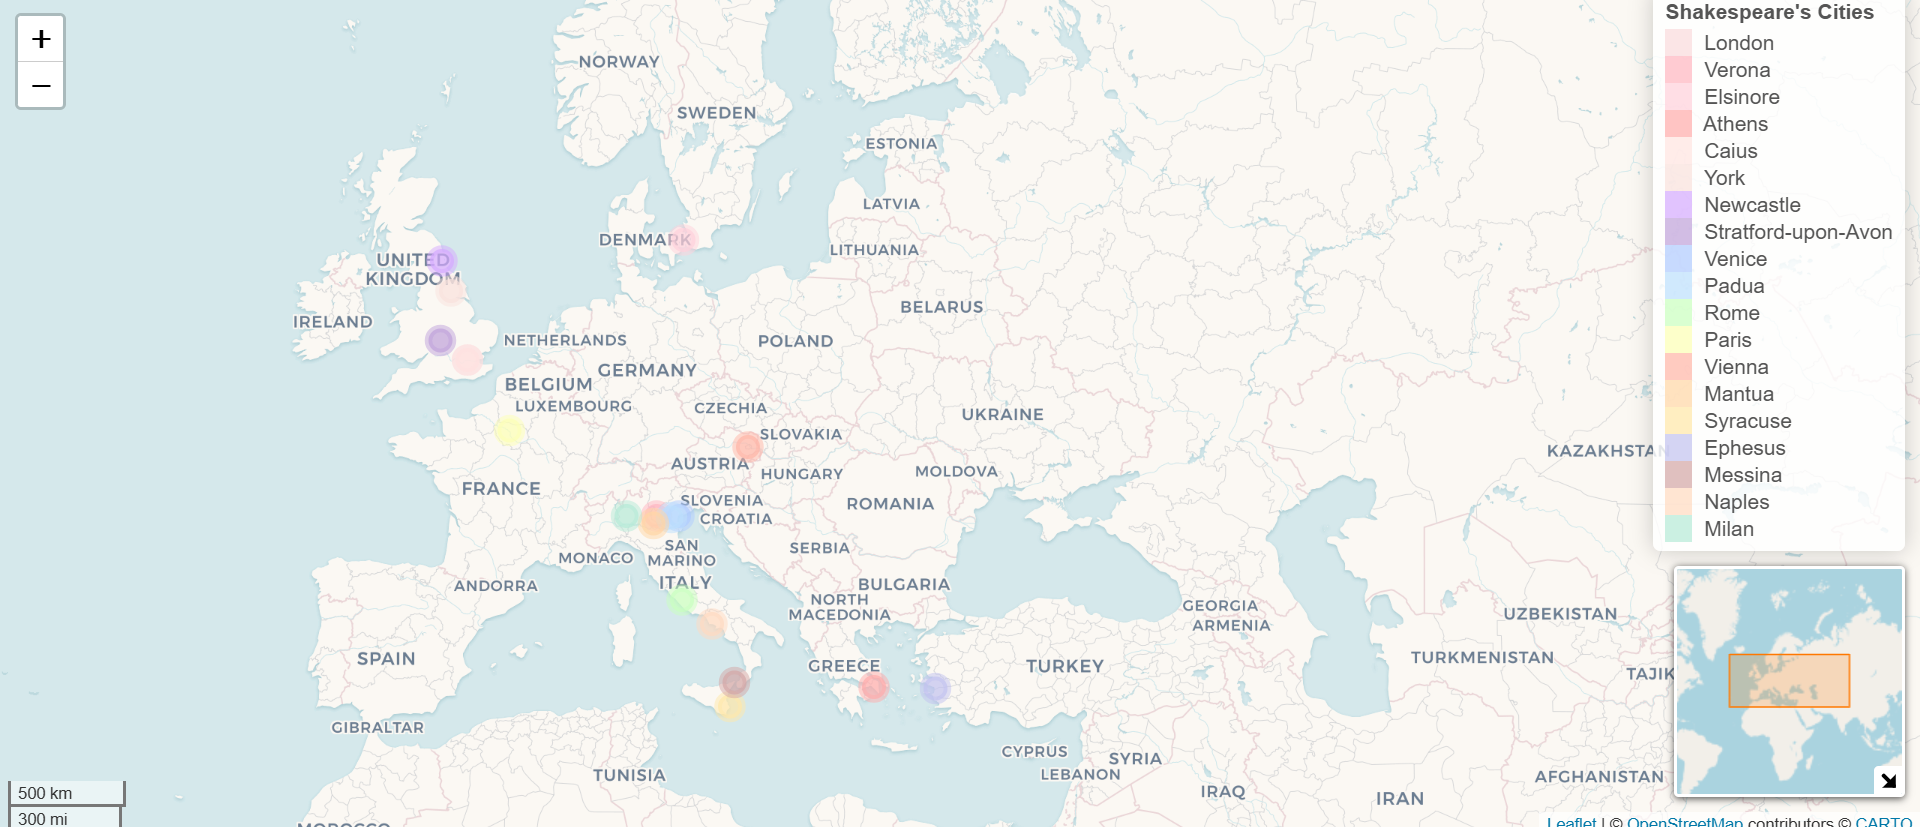
\includegraphics[width=0.8\linewidth]{RStudioMap.png} \\[0.5cm] 
    \textcolor{shakespeareyellow}{\rule{0.8\linewidth}{0.5mm}} 
\end{center}

\vspace{1cm}

\newpage

\section*{\color{shakespeareblue}Visualization of Shakespeare's Cities}
Each city mentioned in Shakespeare's plays was represented on the map as a marker, styled in unique pastel colors for a modern and visually appealing look. The map is interactive, allowing users to click on a marker to see the city's name and its connection to Shakespeare's work. For instance, Verona is prominently featured in \textit{Romeo and Juliet}, while Athens provides the magical backdrop for \textit{A Midsummer Night’s Dream}.

\subsection*{Steps in Creating the Map}

\begin{enumerate}[label=\textcolor{shakespeareblue}{\textbf{\arabic*.}}]
    \item \textbf{Data Collection}: A list of cities mentioned in Shakespeare's plays was compiled, including their geographic coordinates. Each city was grouped into thematic regions to reflect its significance in the plays.
    
    \item \textbf{Building the Map}: Using the \texttt{leaflet} package in \textbf{RStudio}, we plotted each city as a marker, applying pastel colors to ensure that each location stood out clearly while maintaining a cohesive, elegant design.

    \item \textbf{Interactive Features}: Pop-ups were added to each marker, revealing details about the city when clicked. These features enhance engagement and turn the map into a dynamic, educational tool.

    \item \textbf{Exporting the Map}: To accommodate different audiences:
    \begin{itemize}[label=\textcolor{shakespeareyellow}{\textbullet}]
        \item An interactive version was saved as an HTML file, allowing users to explore the map dynamically.
        \item A static image was exported for inclusion in this report, ensuring accessibility in a non-digital format.
    \end{itemize}
\end{enumerate}

\newpage

\section*{\color{shakespeareblue}Relevance to Shakespeare’s Work}
This visualization highlights Shakespeare’s broad geographical imagination, reflecting the cultural and political curiosity of the Elizabethan era. While Shakespeare himself never traveled abroad, his plays transport audiences to diverse settings—Italy, Denmark, and Greece, among others. These locations often symbolize themes central to his narratives: love, conflict, and transformation.

The map serves as both an educational tool and a creative way to appreciate how Shakespeare wove international settings into his stories, making them timeless and universally resonant.

\section*{\color{shakespeareblue}Including the Visualization}
The map is included below as a static image, offering a snapshot of the geographical spread of Shakespeare’s cities. The interactive version is also available and can be explored further in the accompanying digital files.

\begin{figure}[ht]
    \centering
    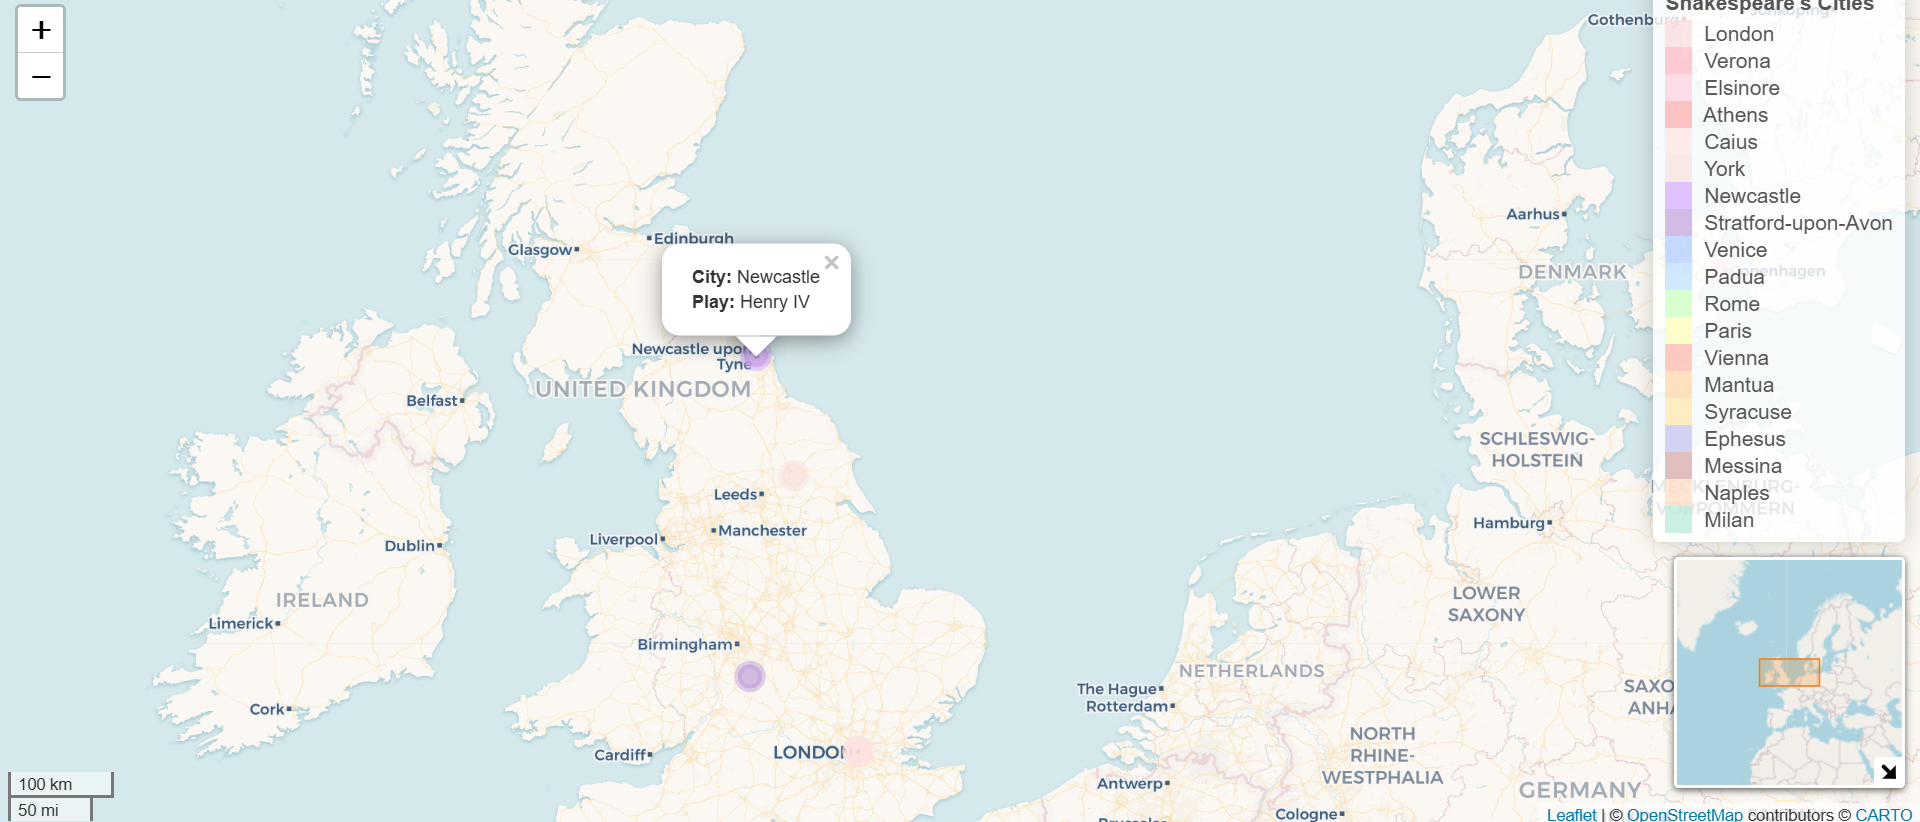
\includegraphics[width=0.8\linewidth]{MapPopUps.png}
    \caption{Static Image of the Interactive Map of Shakespeare's Cities}
    \label{fig:map}
\end{figure}


\section*{\color{shakespeareblue}Conclusion}
The map offers a modern, engaging way to explore the cities referenced in Shakespeare's works. It provides a deeper understanding of his geographical imagination and how he used different locations to enhance the themes and narratives in his plays. Through this visualization, we gain a new appreciation for the diversity of Shakespeare's settings and how they resonate across time and culture.

\newpage
\section*{\color{shakespeareblue}}

\sloppy
\begin{thebibliography}{99}
\raggedright
\bibitem{geonames}
GeoNames. \textit{GeoNames: Geographical Database}. Available at: \url{https://www.geonames.org}. Accessed on January 2025.

\bibitem{folgerpedia}
Folger Shakespeare Library. \textit{List of Settings for Shakespeare's Plays}. Available at: \url{https://folgerpedia.folger.edu/List_of_settings_for_Shakespeare%27s_plays}. Accessed on January 2025.
\end{thebibliography}





\end{document}
